\documentclass[11pt]{article}
\usepackage{amsmath, amssymb, amsthm}
\usepackage{geometry}
\usepackage{graphicx}
\usepackage{hyperref}
\usepackage{cite}
\geometry{margin=1in}
\title{Entropy Collapse and the Quantization of Spacetime:\ A Computational Model of Black Hole Singularity}
\author{Juha}
\date{\today}

\begin{document}
\maketitle

\begin{abstract}
  We present an information-theoretic model of black hole singularities by simulating the evolution of the black hole geometry as a computation model. By representing computational processes as set-theoretic execution traces - bitstrings-, we define a mapping
  from informational states to spacetime geometry. We demonstrate that zero entropy corresponds to a singular point in any
  embedding space. A Python simulation illustrates this entropy-geometry correspondence in dynamic systems.
\end{abstract}

\section{Introduction}

The connection between entropy and geometry is well established in black hole thermodynamics, notably through the Bekenstein--Hawking entropy formula \cite{Bekenstein1973,Hawking1975}, which relates the entropy of a black hole to the surface area of its event horizon. We take this further by considering \emph{entropy collapse}---a transition to a state of minimal information---and its geometric consequence.

This leads to a central claim:

\begin{quote}
  \textbf{Lemma (Entropy--Singularity Lemma):} \emph{Vanishing entropy implies geometric singularity.}
\end{quote}

The paper is structured as follows: we first define the program execution trace using set theory, then describe how such traces map to discrete representations of spacetime. We formalize and defend the lemma and explore its physical consequences.

\section{Methods}

We model the evolution of a black hole spacetime geometry as a set of bitstrings encoding the information in the spacetime. This is accomplished as a simulation where the memory image encoding the spacetime geometry is traced and represented as an ordered set of bitsrings. Even thought the simulation cannot be run to  completion due to  fundamental limits numerical precision, we can analyze the evolution of the bitsrings and extrapolate the simulation to completion using statistical methods. As the simulation
models the qualitative behavior , we hope to gain insight into the nature of black hole singularities and their relationship to entropy.
The simulation is implemented in Python, and the source code is available at \url{http://githumb/juhakm/schwarzchild\_entropy.py}.


\section{Execution Trace in Set-Theoretic Form}

Let $\mathcal{M}$ be the set of all addressable memory units in a machine. Each machine state $s \subseteq \mathcal{M}$ is a subset containing the values of all memory units, registers, and CPU state.

Define $S$ as the set of all possible machine states. Let a program be a finite sequence of instructions:
\[
  P = (I_1, I_2, \dots, I_n)
\]
Each instruction $I_i$ defines a transition function $I_i : S \to S$.

We define the execution trace as an ordered superset of visited states:
\[
  T = (s_0, s_1, \dots, s_n) \quad \text{where } s_{i+1} = I_{i+1}(s_i)
\]

The associated transition relation induced by $P$ is:
\[
  R_P = \{ (s_i, s_{i+1}) \in S \times S \mid s_{i+1} = I_{i+1}(s_i) \}
\]

\section{Mapping Information to Spacetime Geometry}

We represent points in 3D space as triples of integers:
\[
  (x_1, x_2, x_3) \in \mathbb{Z}^3
\]
Each coordinate is derived from a fixed-width binary encoding of simulation data.

Let $b \in \{0,1\}^L$ be a bitstring encoding the complete system state. Let:
\[
  \mathcal{C} = \{0,1\}^{3k}
\]
be the configuration space representing all geometric states under $3k$ bits. Define a mapping:
\[
  f : \mathcal{C} \to \mathbb{Z}^3, \quad f(b) = (\phi(b_1), \phi(b_2), \phi(b_3))
\]
where $\phi : \{0,1\}^k \to \mathbb{Z}$ decodes binary segments.

\section{Entropy Collapse and Geometric Singularity}

Define the empirical frequency $p_T(s)$ over the execution trace $T$:
\[
  H(T) = -\sum_{s \in T} p_T(s) \log_2 p_T(s)
\]

If $H(T) \to 0$, the system visits a single state repeatedly. Any geometric mapping applied to such a system collapses to a single point.

\begin{quote}
  \textbf{Lemma (Entropy--Singularity Lemma):}
  \emph{As Shannon entropy approaches zero, any geometric representation of the corresponding information collapses to a singular point, regardless of encoding or coordinate mapping.}
\end{quote}


\begin{figure}[h!]
  \centering
  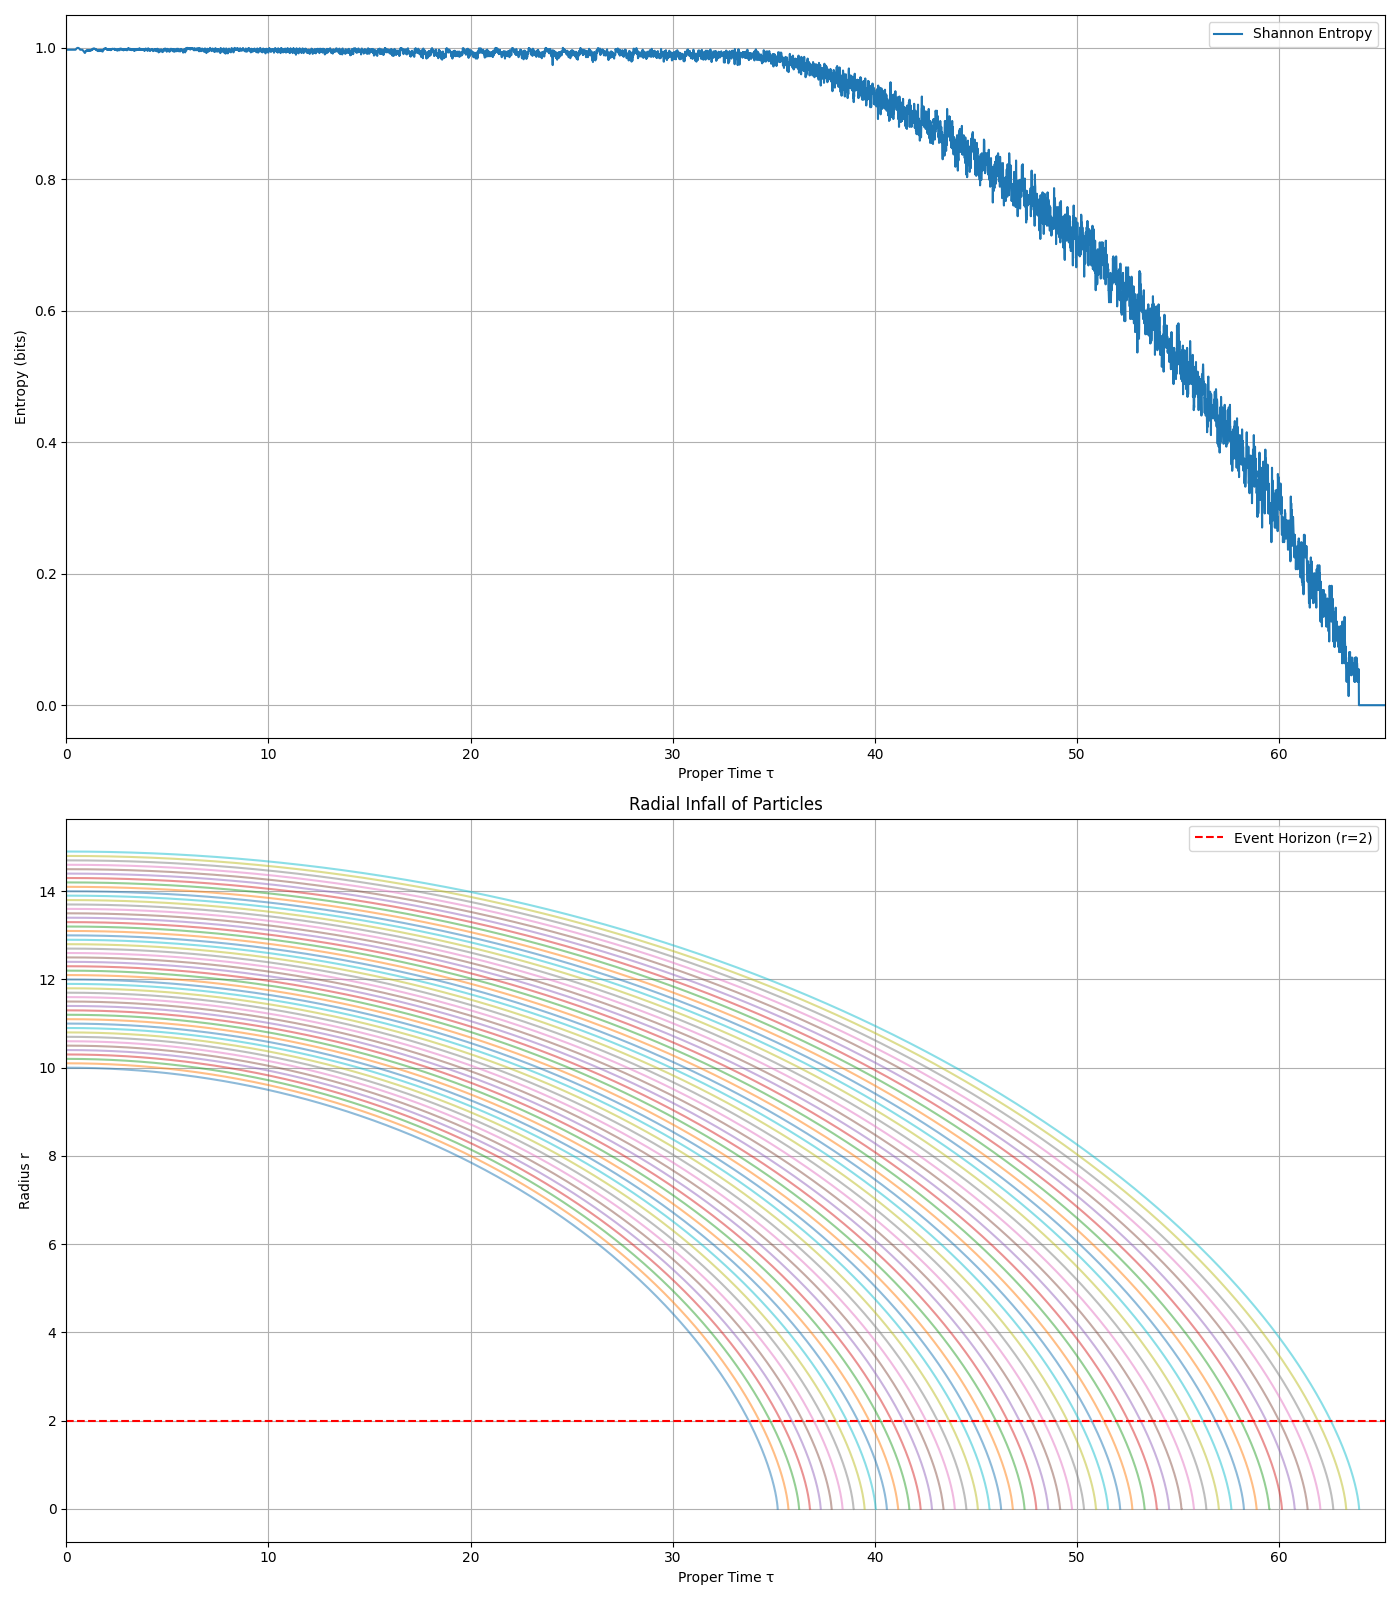
\includegraphics[width=1.0\textwidth]{figures/blackhole_signature.png}
  \caption{Particles falling in Schwarzchild metrics and the corresponding entropy signature of the execution trace. The entropy decreases as the particles approach the singularity, indicating a collapse of information into a point. By extrapolating the entropy signature, we can run the simulation to completion and analyze the properties of the singularity.
      [simulation program \url{http://github.com/juhakm/schwarzchild_entropy.py}]}
  \label{fig:vanishing_entropy}
\end{figure}



\subsection*{Justification}

This result does not depend on the specific method used to interpret a bitstring geometrically. That is, the mapping from information to geometry is irrelevant. Any zero-entropy bitstring consists of repeated or constant values. When mapped to geometric representations---whether through integer decoding, floating-point interpretation, or structured coordinate systems---the lack of informational variability ensures that all resulting points coincide. The outcome is thus a pointlike structure in
any embedding space.

This can be verified empirically. We implemented a brute-force simulation that, given an $n$-bit input, exhaustively generates a variety of geometric interpretations (e.g., integer tuples, floating-point triples, signed encodings) and renders the resulting geometries. When the bitstring has zero entropy (e.g., all zeros or all ones), all interpretations collapse to the same object: a point. This remains true regardless of the internal representation of the data.

\subsection*{Illustrative Example (Python)}

\begin{verbatim}
from itertools import product
import numpy as np
import matplotlib.pyplot as plt

def generate_bitstrings(n):
    return [''.join(bits) for bits in product('01', repeat=n)]

def decode_as_points(bitstring, mode='int', dim=3, chunk_size=8):
    chunks = [bitstring[i:i+chunk_size] for i in range(0, len(bitstring), chunk_size)]
    while len(chunks) < dim:
        chunks.append('0' * chunk_size)
    chunks = chunks[:dim]

    if mode == 'int':
        return tuple(int(c, 2) for c in chunks)
    elif mode == 'float':
        return tuple(int(c, 2)/2**chunk_size for c in chunks)
    else:
        raise ValueError("Unsupported mode")

bitstring = '0' * 24  # zero entropy case
modes = ['int', 'float']
points = []

for mode in modes:
    p = decode_as_points(bitstring, mode=mode)
    points.append(p)

points = np.array(points)
fig = plt.figure()
ax = fig.add_subplot(111, projection='3d')
ax.scatter(points[:,0], points[:,1], points[:,2])
ax.set_title("Geometric interpretations of zero-entropy bitstring")
plt.show()
\end{verbatim}

This validates the assertion that geometric singularity is the universal outcome of vanishing entropy, regardless of encoding scheme or mapping assumptions.


\section{Simulation Details}

We implemented a Python simulation of a collapsing dust cloud. State data was quantized, serialized into bitstrings, and entropy was measured. Over time, bitstring entropy decreased, visually collapsing geometry into a point.

\begin{figure}[h!]
  \centering
  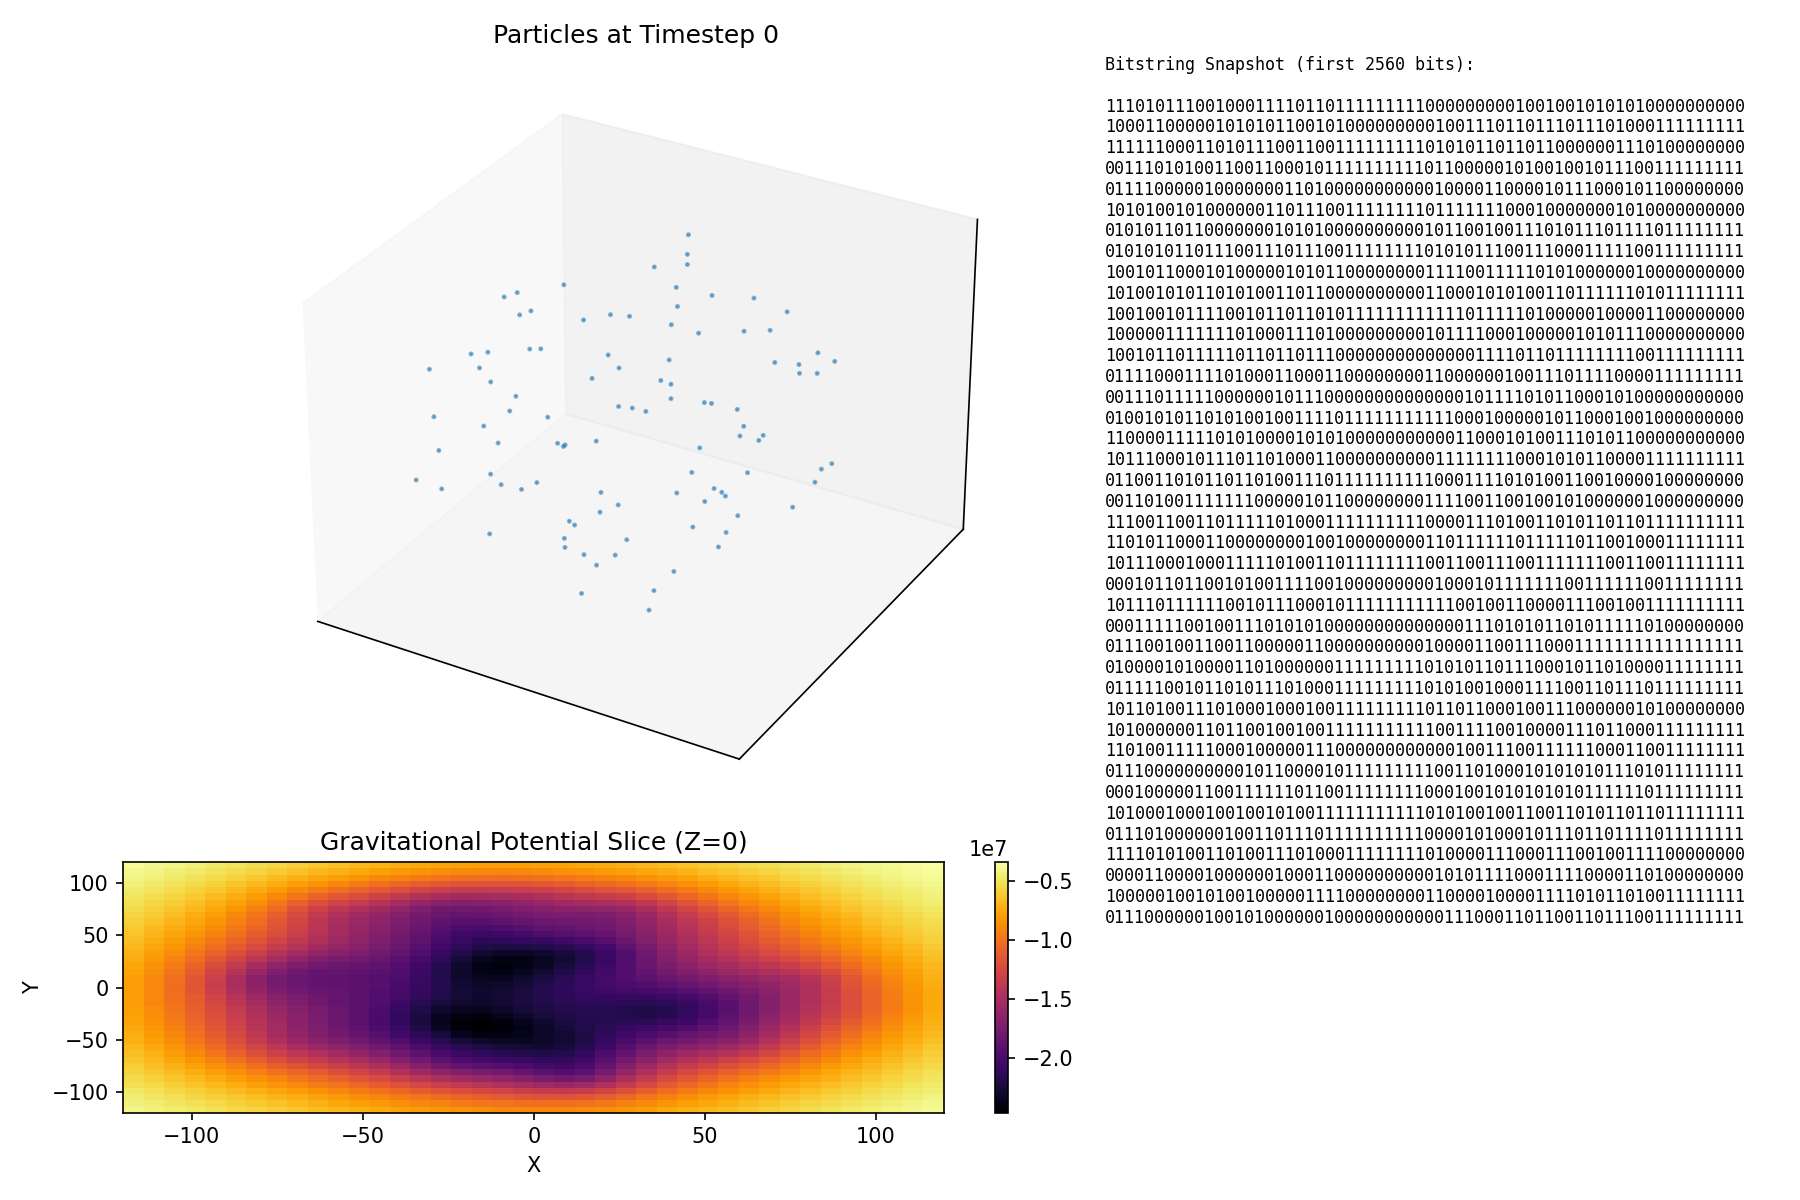
\includegraphics[width=1.0\textwidth]{figures/collapse_0.png}
  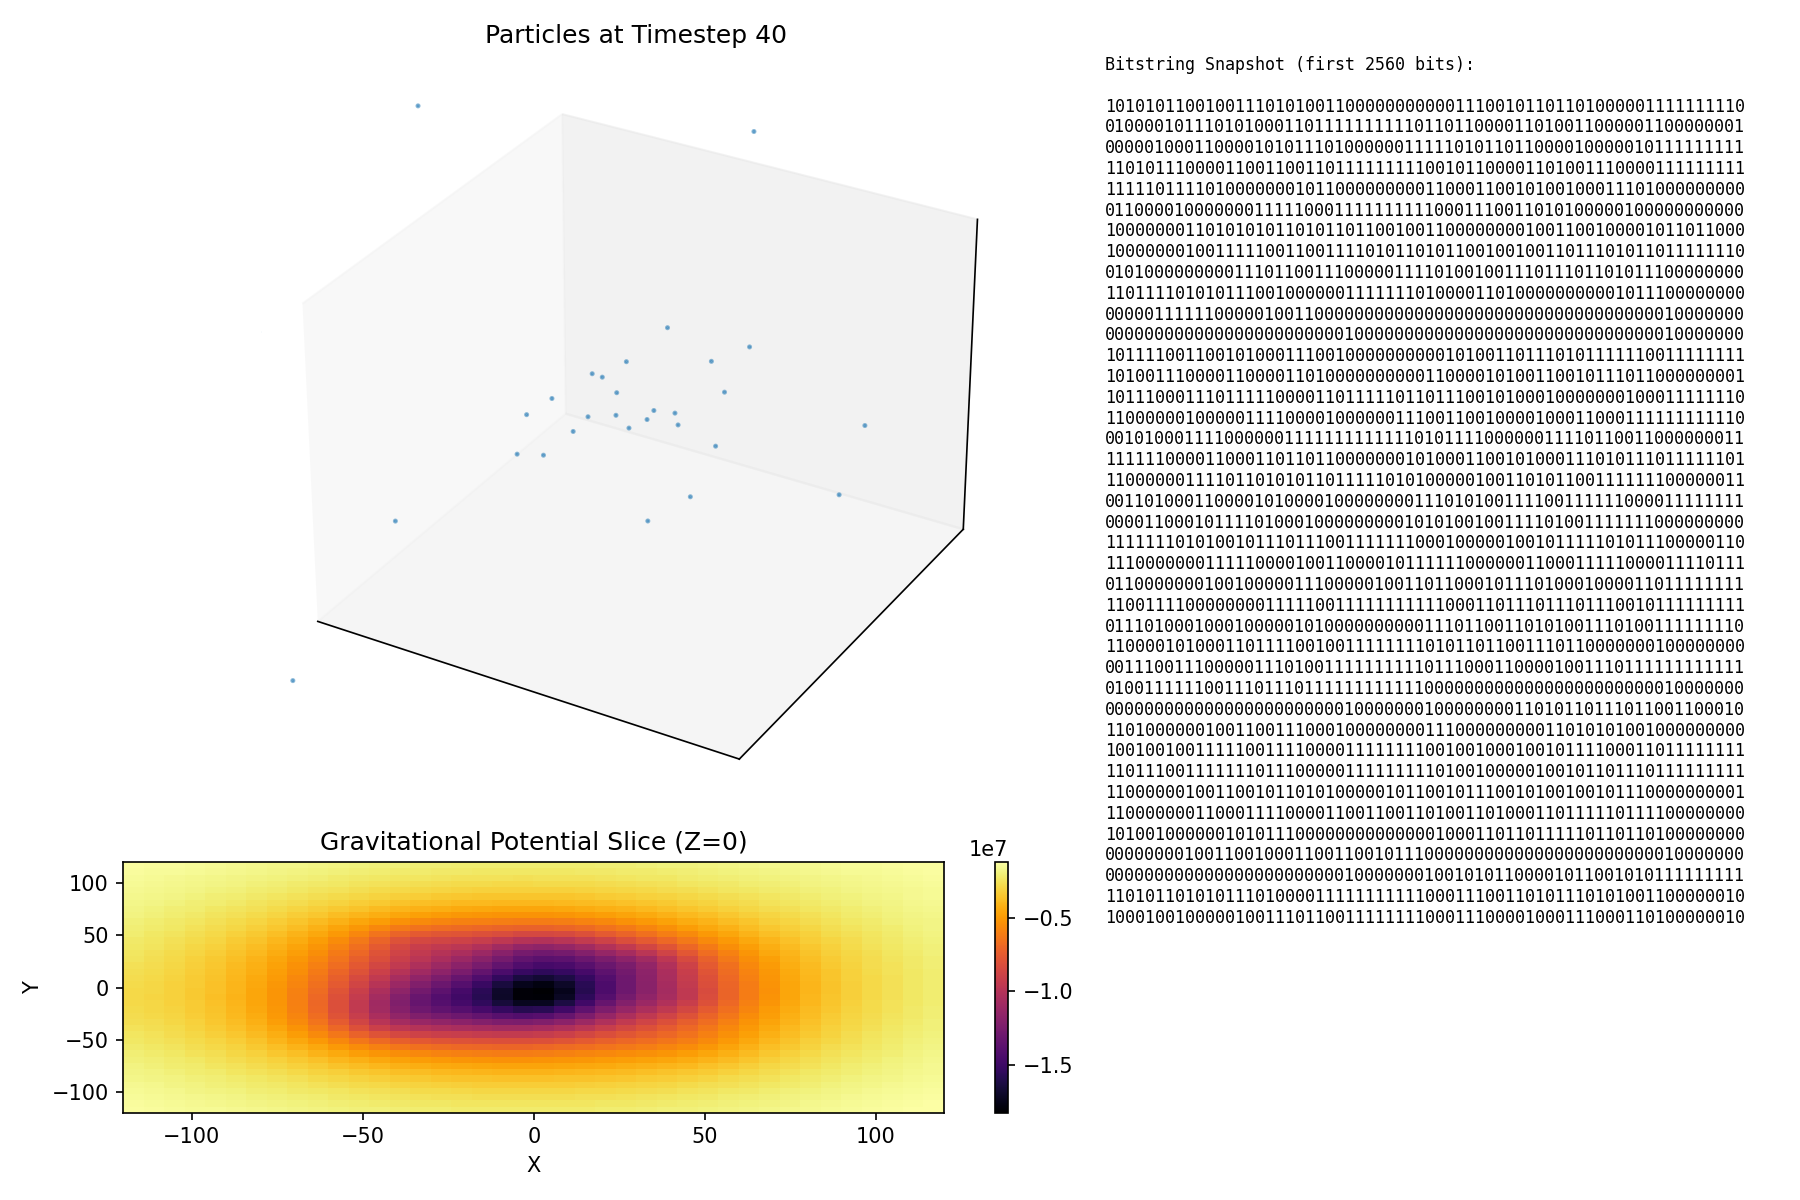
\includegraphics[width=1.0\textwidth]{figures/collapse_40.png}
  \caption{Collapsing spacetime geometry. As entropy decreases, spacetime collapses toward a point.}
  \label{fig:vanishing_entropy}
\end{figure}

\section{Conclusion and Future Work}

We have shown that low-entropy informational states necessarily correspond to geometric singularities. This creates an absolute informational scale for entropy, anchored at zero. Future work will model entropy increase as emergent spacetime expansion, simulate structure formation, and explore whether entropy acts as a driver of geometric complexity.

\appendix
\section{Appendix: Bitstring Encoding}

\begin{itemize}
  \item Quantize floating point: $\mathbb{R} \to \mathbb{Z}$
  \item Serialize integers to binary
  \item Concatenate to $b \in \{0,1\}^L$
\end{itemize}

Entropy of $b$:
\[
  H(b) = -p_0 \log_2 p_0 - p_1 \log_2 p_1
\]
where $p_0$, $p_1$ are empirical frequencies.

\section*{References}
\begin{thebibliography}{9}
  \bibitem{Bekenstein1973} J. D. Bekenstein, "Black Holes and Entropy," \textit{Phys. Rev. D} \textbf{7}, 2333 (1973).
  \bibitem{Hawking1975} S. W. Hawking, "Particle Creation by Black Holes," \textit{Commun. Math. Phys.} \textbf{43}, 199 (1975).
\end{thebibliography}

\end{document}
